\documentclass[14pt]{extbook}
\usepackage{multicol, enumerate, enumitem, hyperref, color, soul, setspace, parskip, fancyhdr} %General Packages
\usepackage{amssymb, amsthm, amsmath, bbm, latexsym, units, mathtools} %Math Packages
\everymath{\displaystyle} %All math in Display Style
% Packages with additional options
\usepackage[headsep=0.5cm,headheight=12pt, left=1 in,right= 1 in,top= 1 in,bottom= 1 in]{geometry}
\usepackage[usenames,dvipsnames]{xcolor}
\usepackage{dashrule}  % Package to use the command below to create lines between items
\newcommand{\litem}[1]{\item#1\hspace*{-1cm}\rule{\textwidth}{0.4pt}}
\pagestyle{fancy}
\lhead{Progress Quiz 4}
\chead{}
\rhead{Version C}
\lfoot{8448-1521}
\cfoot{}
\rfoot{Fall 2020}
\begin{document}

\begin{enumerate}
\litem{
Construct the lowest-degree polynomial given the zeros below. Then, choose the intervals that contain the coefficients of the polynomial in the form $ax^3+bx^2+cx+d$.\[ \frac{3}{2}, -6, \text{ and } \frac{5}{3} \]\begin{enumerate}[label=\Alph*.]
\item \( a \in [5, 11], b \in [34, 42], c \in [-24, -15], \text{ and } d \in [-99, -85] \)
\item \( a \in [5, 11], b \in [14, 18], c \in [-103, -96], \text{ and } d \in [-99, -85] \)
\item \( a \in [5, 11], b \in [-22, -16], c \in [-103, -96], \text{ and } d \in [-99, -85] \)
\item \( a \in [5, 11], b \in [-41, -32], c \in [-11, -3], \text{ and } d \in [87, 95] \)
\item \( a \in [5, 11], b \in [14, 18], c \in [-103, -96], \text{ and } d \in [87, 95] \)

\end{enumerate} }
\litem{
Describe the zero behavior of the zero $x = 3$ of the polynomial below.\[ f(x) = 6(x - 6)^{10}(x + 6)^{9}(x + 3)^{12}(x - 3)^{7} \]\begin{enumerate}[label=\Alph*.]
\begin{multicols}{2}\item 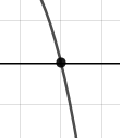
\includegraphics[width = 0.3\textwidth]{../Figures/polyZeroBehaviorCopyAC.png}\item 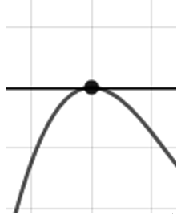
\includegraphics[width = 0.3\textwidth]{../Figures/polyZeroBehaviorCopyBC.png}\item 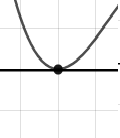
\includegraphics[width = 0.3\textwidth]{../Figures/polyZeroBehaviorCopyCC.png}\item 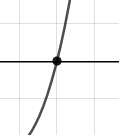
\includegraphics[width = 0.3\textwidth]{../Figures/polyZeroBehaviorCopyDC.png}\end{multicols}\item None of the above.
\end{enumerate} }
\litem{
Construct the lowest-degree polynomial given the zeros below. Then, choose the intervals that contain the coefficients of the polynomial in the form $ax^3+bx^2+cx+d$.\[ 6, 4, \text{ and } \frac{5}{4} \]\begin{enumerate}[label=\Alph*.]
\item \( a \in [4, 8], b \in [-48, -38], c \in [139, 147], \text{ and } d \in [-122, -114] \)
\item \( a \in [4, 8], b \in [-1, 4], c \in [-110, -99], \text{ and } d \in [117, 124] \)
\item \( a \in [4, 8], b \in [-48, -38], c \in [139, 147], \text{ and } d \in [117, 124] \)
\item \( a \in [4, 8], b \in [45, 46], c \in [139, 147], \text{ and } d \in [117, 124] \)
\item \( a \in [4, 8], b \in [29, 37], c \in [42, 52], \text{ and } d \in [-122, -114] \)

\end{enumerate} }
\litem{
Construct the lowest-degree polynomial given the zeros below. Then, choose the intervals that contain the coefficients of the polynomial in the form $x^3+bx^2+cx+d$.\[ -4 + 4 i \text{ and } 2 \]\begin{enumerate}[label=\Alph*.]
\item \( b \in [0, 1.3], c \in [-8, -4], \text{ and } d \in [1, 15] \)
\item \( b \in [0, 1.3], c \in [0, 4], \text{ and } d \in [-15, -3] \)
\item \( b \in [-7.3, -2], c \in [12, 25], \text{ and } d \in [64, 74] \)
\item \( b \in [4.2, 7.3], c \in [12, 25], \text{ and } d \in [-64, -61] \)
\item \( \text{None of the above.} \)

\end{enumerate} }
\litem{
Construct the lowest-degree polynomial given the zeros below. Then, choose the intervals that contain the coefficients of the polynomial in the form $x^3+bx^2+cx+d$.\[ -2 - 5 i \text{ and } 4 \]\begin{enumerate}[label=\Alph*.]
\item \( b \in [-1.34, 0.32], c \in [12.8, 14.7], \text{ and } d \in [113, 118] \)
\item \( b \in [0.71, 1.99], c \in [-2.2, -0.1], \text{ and } d \in [-13, -3] \)
\item \( b \in [-1.34, 0.32], c \in [12.8, 14.7], \text{ and } d \in [-121, -114] \)
\item \( b \in [0.71, 1.99], c \in [-1.7, 1.2], \text{ and } d \in [-24, -19] \)
\item \( \text{None of the above.} \)

\end{enumerate} }
\litem{
Which of the following equations \textit{could} be of the graph presented below?
\begin{center}
    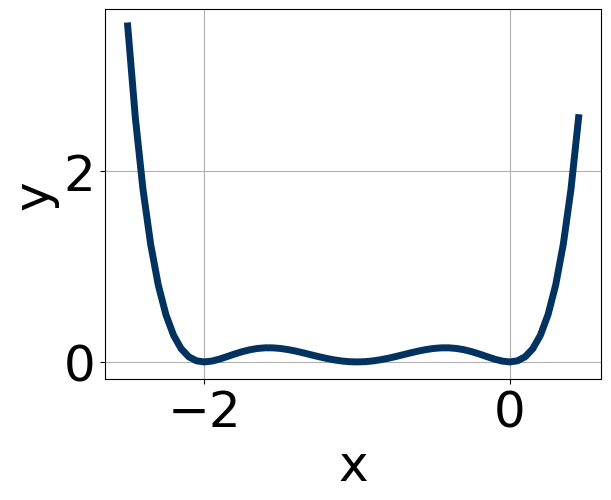
\includegraphics[width=0.5\textwidth]{../Figures/polyGraphToFunctionCopyC.png}
\end{center}
\begin{enumerate}[label=\Alph*.]
\item \( 9x^{6} (x + 4)^{4} (x - 2)^{5} \)
\item \( -17x^{10} (x + 4)^{8} (x - 2)^{9} \)
\item \( -9x^{10} (x + 4)^{7} (x - 2)^{4} \)
\item \( 5x^{10} (x + 4)^{8} (x - 2)^{6} \)
\item \( -10x^{10} (x + 4)^{7} (x - 2)^{9} \)

\end{enumerate} }
\litem{
Which of the following equations \textit{could} be of the graph presented below?
\begin{center}
    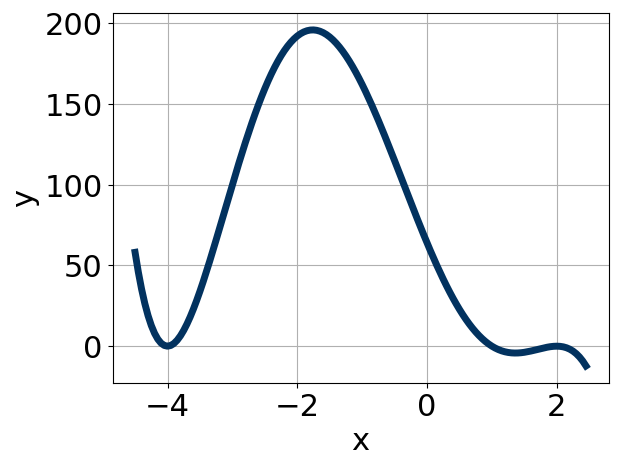
\includegraphics[width=0.5\textwidth]{../Figures/polyGraphToFunctionC.png}
\end{center}
\begin{enumerate}[label=\Alph*.]
\item \( -10(x + 1)^{9} (x + 4)^{8} (x - 2)^{9} \)
\item \( -16(x + 1)^{6} (x + 4)^{6} (x - 2)^{5} \)
\item \( 12(x + 1)^{4} (x + 4)^{9} (x - 2)^{7} \)
\item \( 5(x + 1)^{8} (x + 4)^{5} (x - 2)^{10} \)
\item \( -16(x + 1)^{4} (x + 4)^{9} (x - 2)^{9} \)

\end{enumerate} }
\litem{
Describe the end behavior of the polynomial below.\[ f(x) = -4(x - 4)^{2}(x + 4)^{7}(x - 7)^{3}(x + 7)^{4} \]\begin{enumerate}[label=\Alph*.]
\begin{multicols}{2}\item 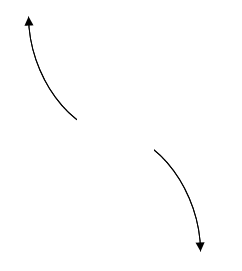
\includegraphics[width = 0.3\textwidth]{../Figures/polyEndBehaviorAC.png}\item 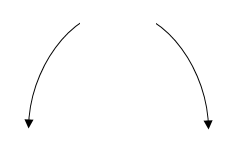
\includegraphics[width = 0.3\textwidth]{../Figures/polyEndBehaviorBC.png}\item 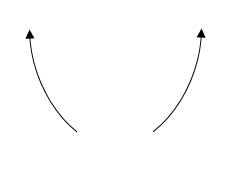
\includegraphics[width = 0.3\textwidth]{../Figures/polyEndBehaviorCC.png}\item 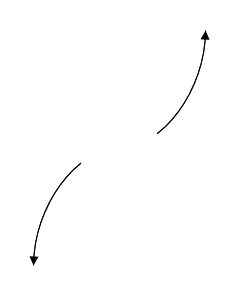
\includegraphics[width = 0.3\textwidth]{../Figures/polyEndBehaviorDC.png}\end{multicols}\item None of the above.
\end{enumerate} }
\litem{
Describe the zero behavior of the zero $x = -3$ of the polynomial below.\[ f(x) = 7(x - 3)^{9}(x + 3)^{10}(x + 4)^{9}(x - 4)^{13} \]\begin{enumerate}[label=\Alph*.]
\begin{multicols}{2}\item 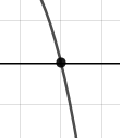
\includegraphics[width = 0.3\textwidth]{../Figures/polyZeroBehaviorAC.png}\item 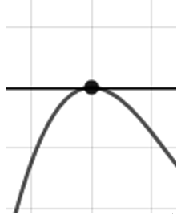
\includegraphics[width = 0.3\textwidth]{../Figures/polyZeroBehaviorBC.png}\item 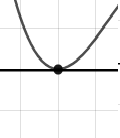
\includegraphics[width = 0.3\textwidth]{../Figures/polyZeroBehaviorCC.png}\item 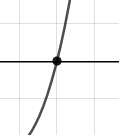
\includegraphics[width = 0.3\textwidth]{../Figures/polyZeroBehaviorDC.png}\end{multicols}\item None of the above.
\end{enumerate} }
\litem{
Describe the end behavior of the polynomial below.\[ f(x) = 2(x + 4)^{2}(x - 4)^{5}(x + 2)^{3}(x - 2)^{5} \]\begin{enumerate}[label=\Alph*.]
\begin{multicols}{2}\item 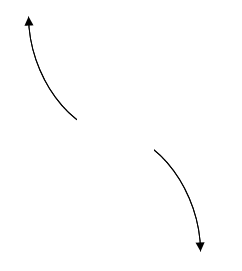
\includegraphics[width = 0.3\textwidth]{../Figures/polyEndBehaviorCopyAC.png}\item 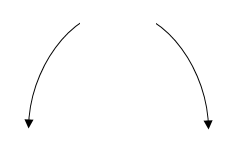
\includegraphics[width = 0.3\textwidth]{../Figures/polyEndBehaviorCopyBC.png}\item 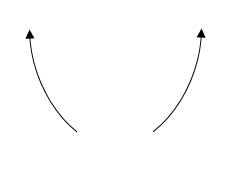
\includegraphics[width = 0.3\textwidth]{../Figures/polyEndBehaviorCopyCC.png}\item 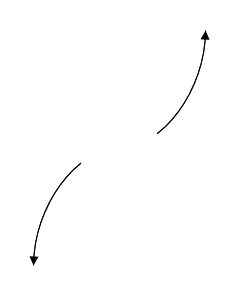
\includegraphics[width = 0.3\textwidth]{../Figures/polyEndBehaviorCopyDC.png}\end{multicols}\item None of the above.
\end{enumerate} }
\end{enumerate}

\end{document}